% Standalone figure for the Statistical Mechanics notes.
% Generated by make_unary_Pv.py (van der Waals isotherms in reduced units).
% Build: pdflatex unary-Pv.tex  (or run build.sh in this folder)
\documentclass[11pt,tikz,border=2pt]{standalone}
\usepackage{amsmath,amssymb}
\usetikzlibrary{arrows.meta, positioning}
\begin{document}
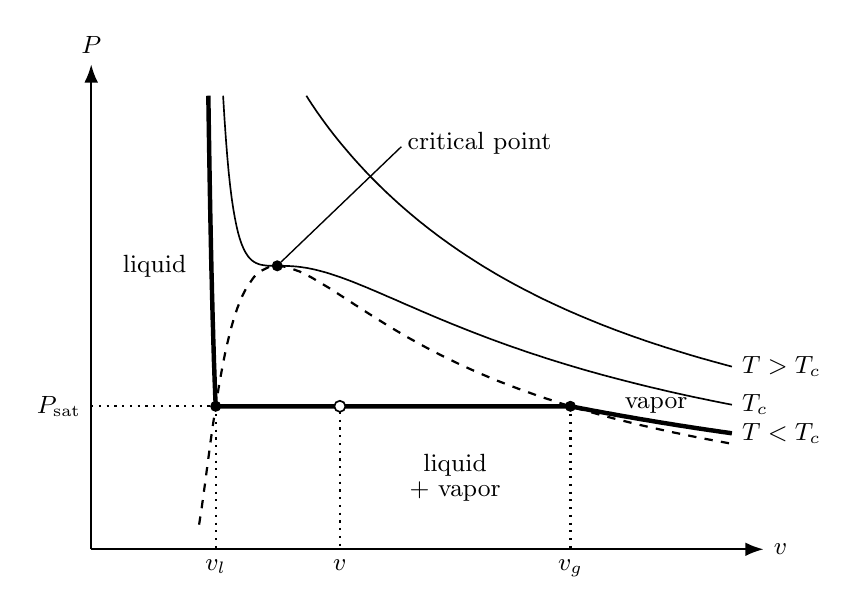
\begin{tikzpicture}[font=\small, >=Latex, line width=0.8pt]
    % axes
    \draw[->] (0,0) -- (8.54,0) node[right] {$v$};
    \draw[->] (0,0) -- (0,6.16) node[above] {$P$};
    % boundary of the two-phase region (coexistence curve)
    \draw[dashed] (1.370,0.313) -- (1.375,0.343) -- (1.380,0.375) -- (1.385,0.409) -- (1.391,0.446) -- (1.397,0.484) -- (1.403,0.524) -- (1.409,0.567) -- (1.415,0.612) -- (1.422,0.659) -- (1.428,0.708) -- (1.435,0.760) -- (1.443,0.814) -- (1.450,0.871) -- (1.458,0.930) -- (1.466,0.992) -- (1.475,1.056) -- (1.483,1.123) -- (1.493,1.192) -- (1.502,1.265) -- (1.512,1.340) -- (1.523,1.417) -- (1.534,1.498) -- (1.546,1.581) -- (1.559,1.667) -- (1.572,1.756) -- (1.586,1.848) -- (1.601,1.943) -- (1.617,2.041) -- (1.634,2.141) -- (1.653,2.245) -- (1.673,2.352) -- (1.695,2.462) -- (1.719,2.575) -- (1.747,2.691) -- (1.777,2.810) -- (1.813,2.933) -- (1.854,3.058) -- (1.905,3.187) -- (1.970,3.319) -- (2.067,3.458) -- (2.143,3.528) -- (2.258,3.586) -- (2.363,3.600) -- (2.480,3.586) -- (2.646,3.528) -- (2.788,3.458) -- (3.021,3.319) -- (3.225,3.187) -- (3.423,3.058) -- (3.619,2.933) -- (3.818,2.810) -- (4.021,2.691) -- (4.231,2.575) -- (4.448,2.462) -- (4.674,2.352) -- (4.910,2.245) -- (5.158,2.141) -- (5.419,2.041) -- (5.693,1.943) -- (5.983,1.848) -- (6.290,1.756) -- (6.615,1.667) -- (6.960,1.581) -- (7.328,1.498) -- (7.720,1.417) -- (8.137,1.340);
    % isotherm above Tc and critical isotherm
    \draw[line width=0.6pt] (2.733,5.760) -- (2.755,5.724) -- (2.778,5.689) -- (2.801,5.653) -- (2.825,5.618) -- (2.848,5.583) -- (2.872,5.548) -- (2.897,5.514) -- (2.921,5.479) -- (2.946,5.445) -- (2.971,5.411) -- (2.996,5.377) -- (3.021,5.343) -- (3.047,5.310) -- (3.073,5.276) -- (3.100,5.242) -- (3.126,5.209) -- (3.153,5.176) -- (3.180,5.143) -- (3.208,5.110) -- (3.236,5.077) -- (3.264,5.044) -- (3.292,5.011) -- (3.321,4.978) -- (3.350,4.945) -- (3.379,4.913) -- (3.409,4.880) -- (3.439,4.848) -- (3.469,4.815) -- (3.499,4.783) -- (3.530,4.751) -- (3.561,4.719) -- (3.593,4.687) -- (3.625,4.655) -- (3.657,4.623) -- (3.690,4.591) -- (3.723,4.559) -- (3.756,4.527) -- (3.790,4.496) -- (3.824,4.464) -- (3.858,4.433) -- (3.893,4.401) -- (3.928,4.370) -- (3.963,4.339) -- (3.999,4.308) -- (4.035,4.277) -- (4.072,4.246) -- (4.109,4.215) -- (4.146,4.184) -- (4.184,4.153) -- (4.223,4.123) -- (4.261,4.092) -- (4.300,4.062) -- (4.340,4.032) -- (4.380,4.001) -- (4.420,3.971) -- (4.461,3.941) -- (4.502,3.912) -- (4.543,3.882) -- (4.586,3.852) -- (4.628,3.823) -- (4.671,3.793) -- (4.714,3.764) -- (4.758,3.735) -- (4.803,3.706) -- (4.848,3.677) -- (4.893,3.648) -- (4.939,3.619) -- (4.985,3.590) -- (5.032,3.562) -- (5.079,3.534) -- (5.127,3.505) -- (5.175,3.477) -- (5.224,3.449) -- (5.273,3.422) -- (5.323,3.394) -- (5.374,3.366) -- (5.425,3.339) -- (5.476,3.312) -- (5.528,3.285) -- (5.581,3.258) -- (5.634,3.231) -- (5.688,3.204) -- (5.742,3.177) -- (5.797,3.151) -- (5.852,3.125) -- (5.908,3.099) -- (5.965,3.073) -- (6.022,3.047) -- (6.080,3.021) -- (6.139,2.996) -- (6.198,2.970) -- (6.258,2.945) -- (6.318,2.920) -- (6.379,2.895) -- (6.441,2.870) -- (6.503,2.845) -- (6.566,2.821) -- (6.630,2.796) -- (6.694,2.772) -- (6.760,2.748) -- (6.825,2.724) -- (6.892,2.700) -- (6.959,2.677) -- (7.027,2.653) -- (7.096,2.630) -- (7.165,2.607) -- (7.235,2.584) -- (7.306,2.561) -- (7.378,2.539) -- (7.450,2.516) -- (7.523,2.494) -- (7.597,2.471) -- (7.672,2.449) -- (7.747,2.427) -- (7.824,2.406) -- (7.901,2.384) -- (7.979,2.363) -- (8.058,2.341) -- (8.137,2.320);
    \draw[line width=0.6pt] (1.675,5.760) -- (1.693,5.465) -- (1.711,5.206) -- (1.729,4.978) -- (1.747,4.779) -- (1.766,4.605) -- (1.785,4.453) -- (1.805,4.321) -- (1.825,4.207) -- (1.845,4.107) -- (1.865,4.022) -- (1.886,3.948) -- (1.907,3.885) -- (1.929,3.832) -- (1.950,3.787) -- (1.973,3.749) -- (1.995,3.717) -- (2.018,3.691) -- (2.041,3.669) -- (2.065,3.652) -- (2.089,3.638) -- (2.114,3.627) -- (2.138,3.618) -- (2.164,3.612) -- (2.190,3.608) -- (2.216,3.604) -- (2.242,3.602) -- (2.269,3.601) -- (2.297,3.600) -- (2.325,3.600) -- (2.353,3.600) -- (2.382,3.600) -- (2.411,3.600) -- (2.441,3.600) -- (2.471,3.599) -- (2.502,3.598) -- (2.534,3.596) -- (2.566,3.594) -- (2.598,3.592) -- (2.631,3.588) -- (2.664,3.584) -- (2.698,3.579) -- (2.733,3.574) -- (2.768,3.567) -- (2.804,3.560) -- (2.840,3.552) -- (2.877,3.543) -- (2.915,3.533) -- (2.953,3.523) -- (2.992,3.512) -- (3.031,3.500) -- (3.071,3.487) -- (3.112,3.473) -- (3.154,3.459) -- (3.196,3.444) -- (3.239,3.428) -- (3.282,3.412) -- (3.326,3.395) -- (3.371,3.377) -- (3.417,3.358) -- (3.464,3.339) -- (3.511,3.320) -- (3.559,3.299) -- (3.608,3.279) -- (3.658,3.257) -- (3.708,3.236) -- (3.759,3.213) -- (3.812,3.191) -- (3.865,3.168) -- (3.919,3.144) -- (3.973,3.120) -- (4.029,3.096) -- (4.086,3.072) -- (4.143,3.047) -- (4.202,3.021) -- (4.262,2.996) -- (4.322,2.970) -- (4.384,2.944) -- (4.446,2.918) -- (4.510,2.892) -- (4.574,2.865) -- (4.640,2.839) -- (4.707,2.812) -- (4.775,2.785) -- (4.844,2.758) -- (4.914,2.731) -- (4.985,2.704) -- (5.058,2.676) -- (5.132,2.649) -- (5.206,2.622) -- (5.283,2.594) -- (5.360,2.567) -- (5.439,2.540) -- (5.519,2.512) -- (5.600,2.485) -- (5.683,2.458) -- (5.767,2.430) -- (5.853,2.403) -- (5.940,2.376) -- (6.028,2.349) -- (6.118,2.322) -- (6.209,2.295) -- (6.302,2.268) -- (6.396,2.242) -- (6.492,2.215) -- (6.590,2.189) -- (6.689,2.163) -- (6.790,2.137) -- (6.892,2.111) -- (6.996,2.085) -- (7.102,2.059) -- (7.210,2.034) -- (7.319,2.008) -- (7.430,1.983) -- (7.543,1.958) -- (7.658,1.933) -- (7.775,1.909) -- (7.894,1.884) -- (8.015,1.860) -- (8.137,1.836);
    % isotherm below Tc: liquid branch, two-phase segment, vapor branch
    \draw[line width=1.6pt] (1.488,5.760) -- (1.489,5.657) -- (1.491,5.555) -- (1.492,5.456) -- (1.494,5.357) -- (1.495,5.260) -- (1.497,5.165) -- (1.498,5.072) -- (1.500,4.979) -- (1.501,4.889) -- (1.503,4.799) -- (1.504,4.712) -- (1.506,4.625) -- (1.507,4.540) -- (1.509,4.456) -- (1.510,4.374) -- (1.512,4.293) -- (1.513,4.213) -- (1.515,4.134) -- (1.517,4.057) -- (1.518,3.981) -- (1.520,3.906) -- (1.521,3.833) -- (1.523,3.761) -- (1.524,3.689) -- (1.526,3.619) -- (1.527,3.550) -- (1.529,3.483) -- (1.531,3.416) -- (1.532,3.350) -- (1.534,3.286) -- (1.535,3.222) -- (1.537,3.160) -- (1.539,3.098) -- (1.540,3.038) -- (1.542,2.978) -- (1.543,2.920) -- (1.545,2.863) -- (1.547,2.806) -- (1.548,2.750) -- (1.550,2.696) -- (1.551,2.642) -- (1.553,2.589) -- (1.555,2.537) -- (1.556,2.486) -- (1.558,2.436) -- (1.559,2.386) -- (1.561,2.338) -- (1.563,2.290) -- (1.564,2.243) -- (1.566,2.197) -- (1.568,2.152) -- (1.569,2.107) -- (1.571,2.063) -- (1.573,2.020) -- (1.574,1.978) -- (1.576,1.937) -- (1.578,1.896) -- (1.579,1.856) -- (1.581,1.816) -- (6.086,1.816) -- (6.115,1.810) -- (6.145,1.805) -- (6.175,1.799) -- (6.205,1.793) -- (6.236,1.787) -- (6.266,1.782) -- (6.297,1.776) -- (6.327,1.770) -- (6.358,1.764) -- (6.389,1.758) -- (6.421,1.753) -- (6.452,1.747) -- (6.484,1.741) -- (6.515,1.735) -- (6.547,1.729) -- (6.579,1.724) -- (6.612,1.718) -- (6.644,1.712) -- (6.677,1.706) -- (6.710,1.700) -- (6.743,1.694) -- (6.776,1.688) -- (6.809,1.683) -- (6.843,1.677) -- (6.876,1.671) -- (6.910,1.665) -- (6.944,1.659) -- (6.978,1.653) -- (7.013,1.647) -- (7.048,1.642) -- (7.082,1.636) -- (7.117,1.630) -- (7.153,1.624) -- (7.188,1.618) -- (7.224,1.612) -- (7.259,1.606) -- (7.295,1.601) -- (7.331,1.595) -- (7.368,1.589) -- (7.404,1.583) -- (7.441,1.577) -- (7.478,1.571) -- (7.515,1.566) -- (7.552,1.560) -- (7.590,1.554) -- (7.628,1.548) -- (7.666,1.542) -- (7.704,1.536) -- (7.742,1.531) -- (7.781,1.525) -- (7.820,1.519) -- (7.859,1.513) -- (7.898,1.508) -- (7.937,1.502) -- (7.977,1.496) -- (8.017,1.490) -- (8.057,1.485) -- (8.097,1.479) -- (8.137,1.473);
    % critical point
    \fill (2.363,3.600) circle (2pt);
    \draw[line width=0.5pt] (2.413,3.650) -- (3.938,5.112);
    \node[right] at (3.888,5.162) {critical point};
    % coexisting volumes, overall state and saturation pressure
    \fill (1.581,1.816) circle (2pt);
    \fill (6.086,1.816) circle (2pt);
    \filldraw[fill=white, line width=0.6pt] (3.158,1.816) circle (2pt);
    \draw[dotted] (1.581,1.816) -- (1.581,0) node[below] {$v_l$};
    \draw[dotted] (3.158,1.746) -- (3.158,0) node[below] {$v$};
    \draw[dotted] (6.086,1.816) -- (6.086,0) node[below] {$v_g$};
    \draw[dotted] (0,1.816) -- (1.581,1.816);
    \node[left] at (0,1.816) {$P_{\text{sat}}$};
    % phase labels
    \node[left] at (1.338,3.600) {liquid};
    \node[align=center] at (4.622,0.908) {liquid\\[-2pt]$+$ vapor};
    \node at (7.175,1.831) {vapor};
    % isotherm labels
    \node[right] at (8.137,1.473) {$T<T_c$};
    \node[right] at (8.137,1.836) {$T_c$};
    \node[right] at (8.137,2.320) {$T>T_c$};
\end{tikzpicture}
\end{document}
